
\chapter{Теоретичні засади проблеми}\label{sec:First}

\section{Характеристики ракетного двигуна. Основні параметри РРД}

Ракетний двигун є пристроєм, що забезпечує рух літального апарата за рахунок сили, яка виникає внаслідок відкидання маси певного робочого тіла, що має кінетичну енергію. Ця сила називається \emph{реактивною тягою}; вона виражається наступним чином:

\begin{equation*}
	\vec{P} =m_{r}\vec{a} ,
\end{equation*}
де $\vec{P}$ --- тяга, $m_r$ --- маса літального апарата, $a$ --- результуюче прискорення. В альтернативному вигляді цей вираз має назву рівняння Мещерського:
\begin{equation*}
	\vec{P} = - \vec{u} \dot{m}_f,
\end{equation*}

де $\vec u$ ---  швидкість витікання РТ, $\dot{m}_f$ --- масова витрата РТ.

Реактивна тяга є наслідком виконання закону збереження імпульсу у системі ''літальний апарат -- робоче тіло РД '' ~\cite{Sivuhin}. Точкою прикладання цієї сили вважають центр зрізу сопла двигуна, а її вектор є протилежним до вектору швидкості витікання робочого тіла.

Другою основною характеристикою ракетного двигуна є питомий імпульс (англ. specific impulse) --- відношення тяги до масової витрати РТ:

\begin{equation*}
    I_{sp} = \frac{P}{\dot{m}},
\end{equation*}
де  $I_{sp}$ ---  питомий імпульс, $P$ ---  тяга, $m$ --- витрата РТ. 

Питомий імпульс є характеристикою ефективності перетворення енергії витікаючого робочого тіла у кінетичну енергію руху літального апарата. В ідеальному випадку питомий імпульс дорівнює ефективній швидкості витікання робочого тіла; на практиці вони відрізняються внаслідок втрати кінетичної енергії під час проміжних перетворень~\cite[с. 16 -- 23]{Alemasov}~\cite[с. 53]{Sutton}. 

Окрім цього важливими параметрами, що визначають характеристики хімічного РД, є витратний комплекс, тяговий комплекс та ступінь розширення сопла.

Витратним комплексом є співвідношення виду:

\begin{equation*}
	\beta = \frac{p_{ch} F^{*}}{\dot{m}},
\end{equation*}
де  $p_{ch}$ ---  тиск у камері згоряння, $F^{*}$ ---  площа критики, $\dot{m}$ --- масова витрата РТ.

Витратний комплекс є характеристикою, що визначає ефективність роботи камери згоряння РД безпосередньо, не враховуючи вплив сопла. Також вона визначає ступінь досконалості підібраної паливної суміші (пального і окиснювача у певному співвідношенні).

Іншою характеристикою ракетного двигуна є тяговий комплекс (коефіцієнт тяги), що виражається як:

\begin{equation*}
K_{p} = \frac{P}{p_{ch} F^{*}}
\end{equation*}

де  $P$ ---  сумарна тяга двигуна, $p_{ch}$ ---  тиск у камері згоряння, $F^{*}$ ---  площа критики.

Тяговий комплекс визначає відношення усієї тяги двигуна до складової тяги, яку створює камера згоряння.

Питомий імпульс хімічного РРД пов'язаний з витратним та тяговим комплексом співвідношенням:

\begin{equation*}
	 I_{sp} = \beta K_{p}
\end{equation*}

Геометричний ступінь розширення сопла визначає основні його параметри: відношення тиску у критичному перерізі до тиску на його крайовому перерізі (зрізі сопла), число Маха у газовому потоці на виході з двигуна тощо. Він дорівнює відношенню:

\begin{equation*}
	\epsilon = \frac{F_{e}}{F^{*}}
\end{equation*}

де  $F_{e}$ ---  площа зрізу сопла, $F^{*}$ ---  площа критики.

Наведені параметри є основними характеристиками, що використовуються для опису роботи рідинних ракетних двигунів~\cite[с. 20 -- 23]{Dobrovolskiy}.
 
 
\section{Базові цикли ракетних двигунів і їх характеристика}

Існує багато видів та підвидів ракетних двигунів. Кожен з них має свої особливості, але усі вони об’єднані у 3 типи: хімічні, ядерні та електричні. 

Найбільш поширені хімічні ракетні двигуни, в яких, в результаті екзотермічної хімічної реакції пального і окиснювача (разом називаються паливом), продукти згоряння нагріваються в камері згоряння до високих температур, розширюючись, розганяються в надзвуковому соплі і витікають з двигуна. Паливо хімічного ракетного двигуна є джерелом як теплової енергії, так і газоподібного робочого тіла, при розширенні якого його внутрішня енергія перетворюється в кінетичну енергію реактивного струменя. Хімічні двигуни мають на даний момент найбільшу тягу серед РД, але вони мають малий питомий імпульс, тому витрата палива у цих двигунів дуже висока; їхня ефективність змінюється при різних значеннях тиску, тому на етапі виходу з верхніх шарів атмосфери двигун є занадто витратним.

Ядерний ракетний двигун --- реактивний двигун, робоче тіло в якому (наприклад, водень, аміак та ін.) нагрівається за рахунок енергії, що виділяється при ядерних реакціях (розпаду або термоядерного синтезу). Розрізняють ядерні та термоядерні ракетні двигуни. ЯРД за агрегатним станом ядерного палива в них поділяються на твердо-, рідинно- і газофазні. У твердофазних ЯРД речовина, яка ділиться, як і в звичайних ядерних реакторах, розміщена в збірках --- стрижнях (ТВЕЛах) складної форми з розвиненою поверхнею, що дозволяє ефективно нагрівати (променистою енергією в даному випадку можна знехтувати) газоподібне робоче тіло (зазвичай --- водень, рідше --- аміак), що одночасно є теплоносієм, охолоджуючим елементи конструкції і самі збірки~\cite[с. 11 -- 12]{Koroteyev}. Існують проекти потужних ядерних двигунів, які на даний момент є єдиним економічним та доступним рішенням проблеми пілотованих експедицій на Місяць і Марс, але можливості сучасних ЯРД сильно обмежені параметрами матеріалів, що використовуються в конструкції активної зони, до того ж велика кількість запусків КА з такими двигунами може сильно погіршити екологічну ситуацію; окрім того, відпрацьовані установки потрібно буде утилізувати.

В електричних ракетних двигунах (ЕРД) як джерело енергії для створення тяги використовується електрична енергія. Питомий імпульс електричних ракетних двигунів може досягати $200$~км/с. Залежно від способу перетворення електричної енергії в кінетичну енергію реактивного струменя, розрізняють електротермічні ракетні двигуни, електростатичні (іонні) ракетні двигуни і електромагнітні ракетні двигуни. У електротермічному РД електрична енергія застосовується для нагріву робочого тіла (РТ) з метою звернення його в газ з температурою $1000 - 5000$~К; газ, витікаючи з реактивного сопла (аналогічного соплу хімічного РД), створює тягу. У електростатичному РД, наприклад іонному, спочатку проводиться іонізація РТ, після чого позитивні іони прискорюються в електростатичному полі (за допомогою системи електродів) і, витікаючи з сопла, створюють тягу (для нейтралізації заряду реактивного струменя в неї інжектуються електрони). З-поміж усіх ЕРД вирізняють плазмові ракетні двигуни, робоче тіло яких набуває прискорення, перебуваючи в стані плазми. Електричні двигуни мають великий питомий імпульс та ресурс роботи, але їх тяга є надто малою для використання в апаратах, які працюють в межах системи <<Земля-Місяць>>.

Варто детальніше розглянути такий тип хімічних ракетних двигунів, як рідинні, оскільки вони ретельно розглядатимуться нижче.
Принцип роботи рідинного ракетного двигуна з насосною подачею компонентів палива можна описати наступним чином (рис.~\ref{fig:SSME}).

\begin{figure}
    \centering
    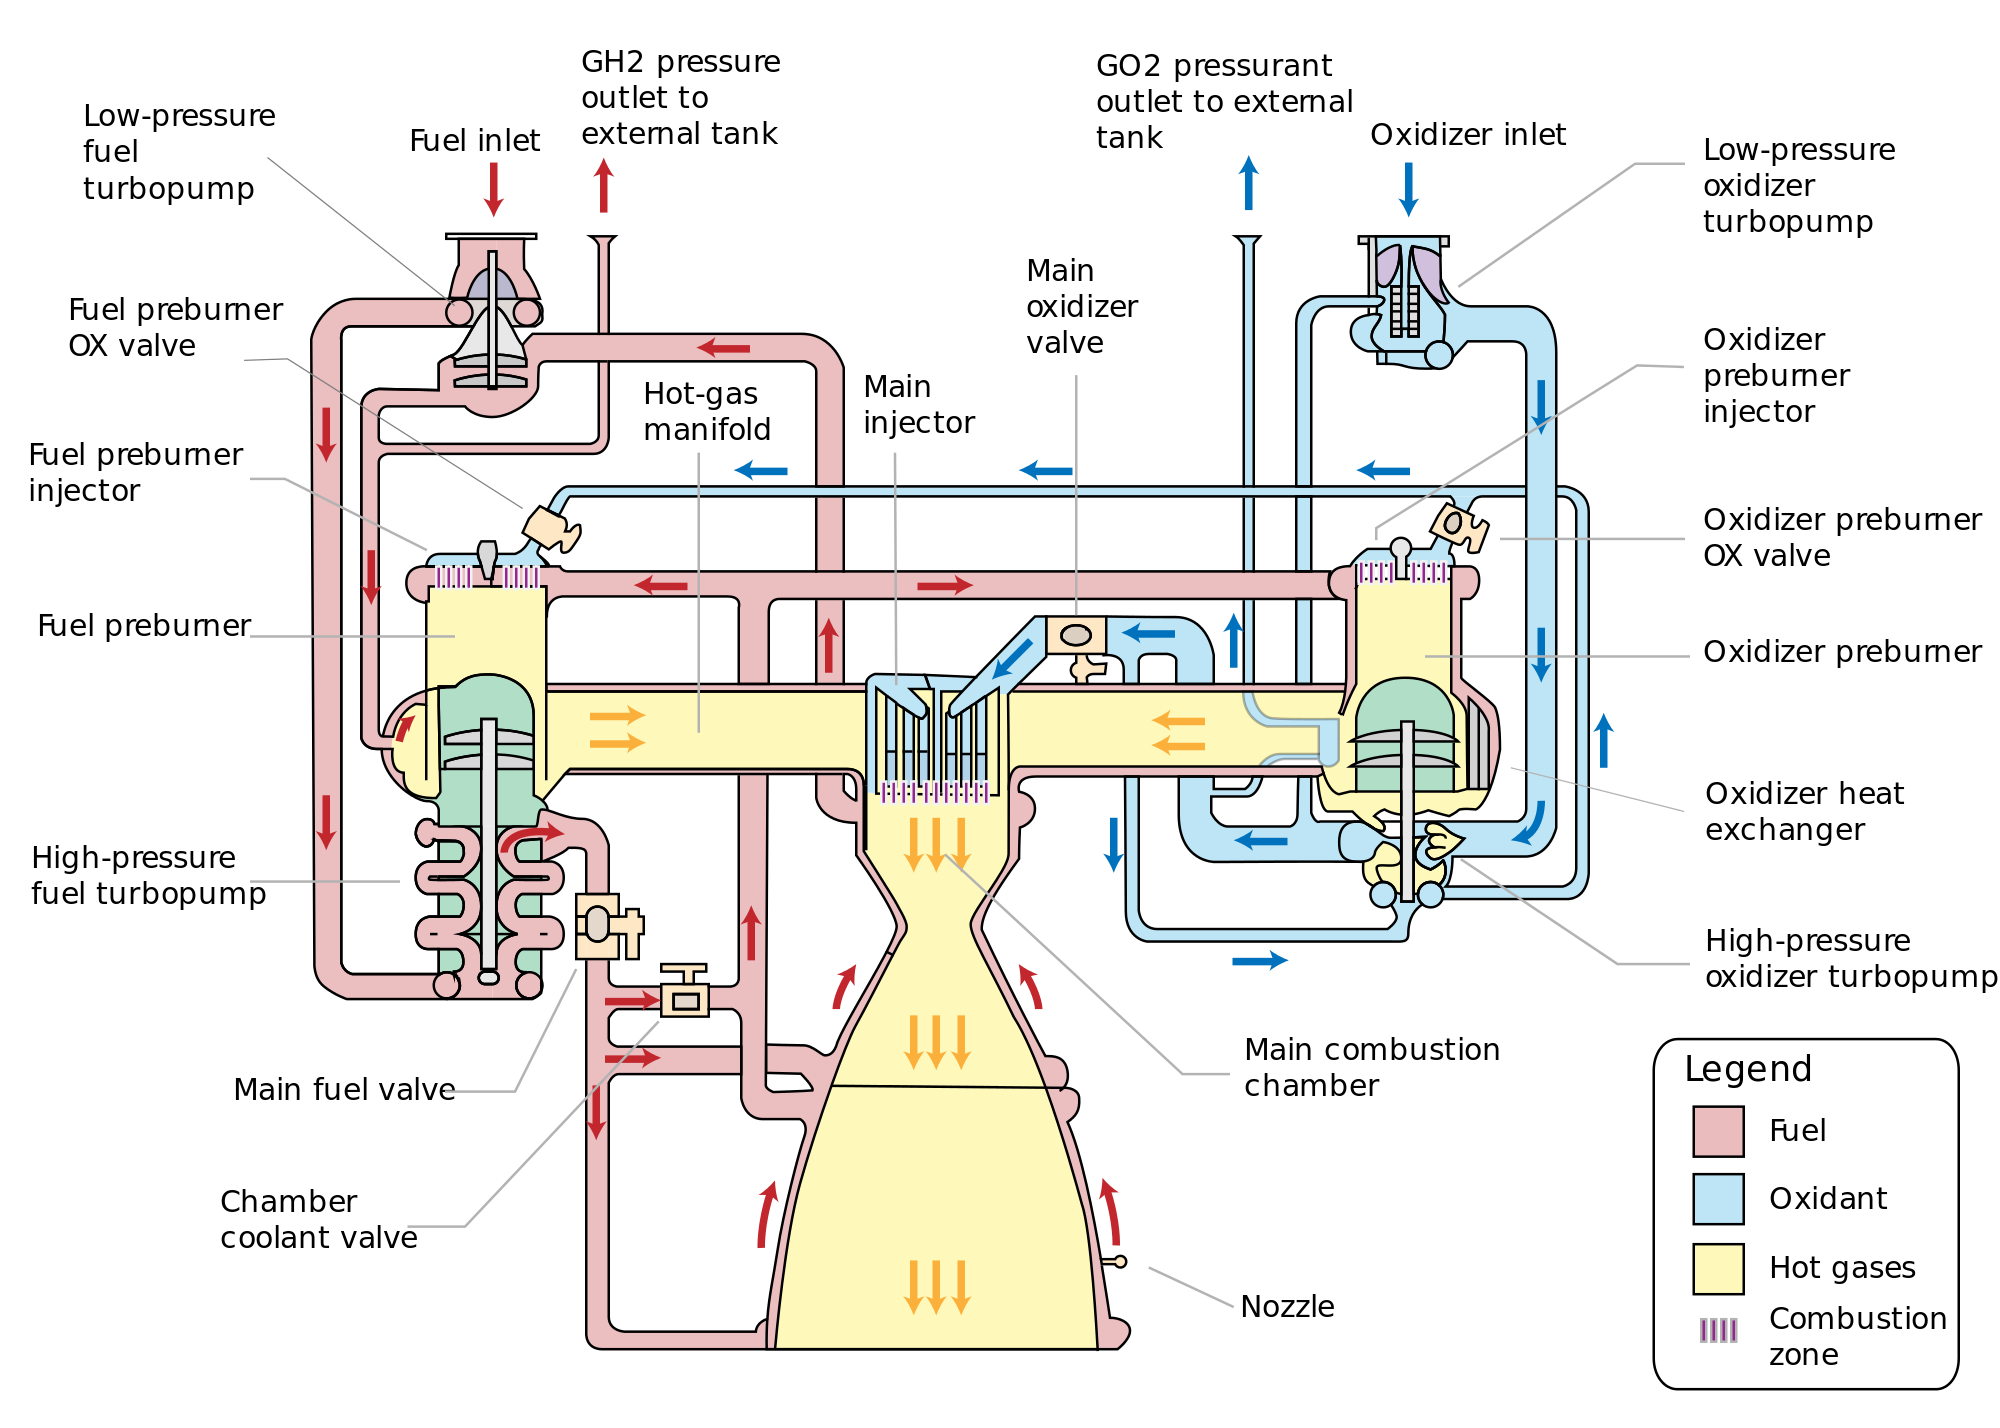
\includegraphics[width=0.6\textheight, angle=0,origin=c]{chapter_1/Ssme_schematic_(updated).svg.png}
    \caption{Умовна схема роботи РРД RS-25 з насосною подачею компонентів палива}
    \label{fig:SSME}
\end{figure}

Компоненти палива --- паливо і окиснювач надходять з баків на відцентрові насоси, що приводяться в рух газовою турбіною. Під високим тиском компоненти палива надходять на форсункову головку  --- вузол, в якому розміщені форсунки, через які компоненти нагнітаються в камеру згоряння, перемішуються і згорають, створюючи нагріте до високої температури газоподібне робоче тіло, яке, розширюючись у соплі, здійснює роботу і перетворює внутрішню енергію газу в кінетичну енергію його направленого руху. Через сопло газ виходить з великою швидкістю, надаючи двигуну реактивну тягу.

Паливна система РРД складається з елементів, що використовуються для подачі палива в камеру згоряння — паливних баків, трубопроводів, турбонасосного агрегату — вузла, що складається з насосів і турбіни, змонтованих на єдиному валу, форсункової голівки і клапанів, які регулюють подачу палива. Насосна подача палива дозволяє створити в камері двигуна високий тиск, від десятків до сотень атмосфер. Високий тиск забезпечує більший ступінь розширення робочого тіла, що є передумовою для досягнення високого значення питомого імпульсу. Крім того, при великому тиску в камері згоряння досягається краще значення тягооснащеності двигуна — відношення величини тяги до маси двигуна. Чим більше значення цього показника, тим менше розміри і маса двигуна (за тієї ж тяги), і тим вище ступінь його досконалості. Переваги насосної системи особливо позначаються в РРД з великою тягою --- наприклад, у рушійних установках ракет-носіїв.

Відпрацьовані гази з турбіни ТНА надходять через форсункову голівку в камеру згоряння разом з компонентами палива. Такий двигун називається двигуном із замкнутим циклом (інакше — з закритим циклом), при якому усе витрачене паливо, включаючи використовуване в приводі ТНА, проходить через камеру згоряння РРД (рис.~\ref{fig:closed_cycle}).

\begin{figure}
    \centering
    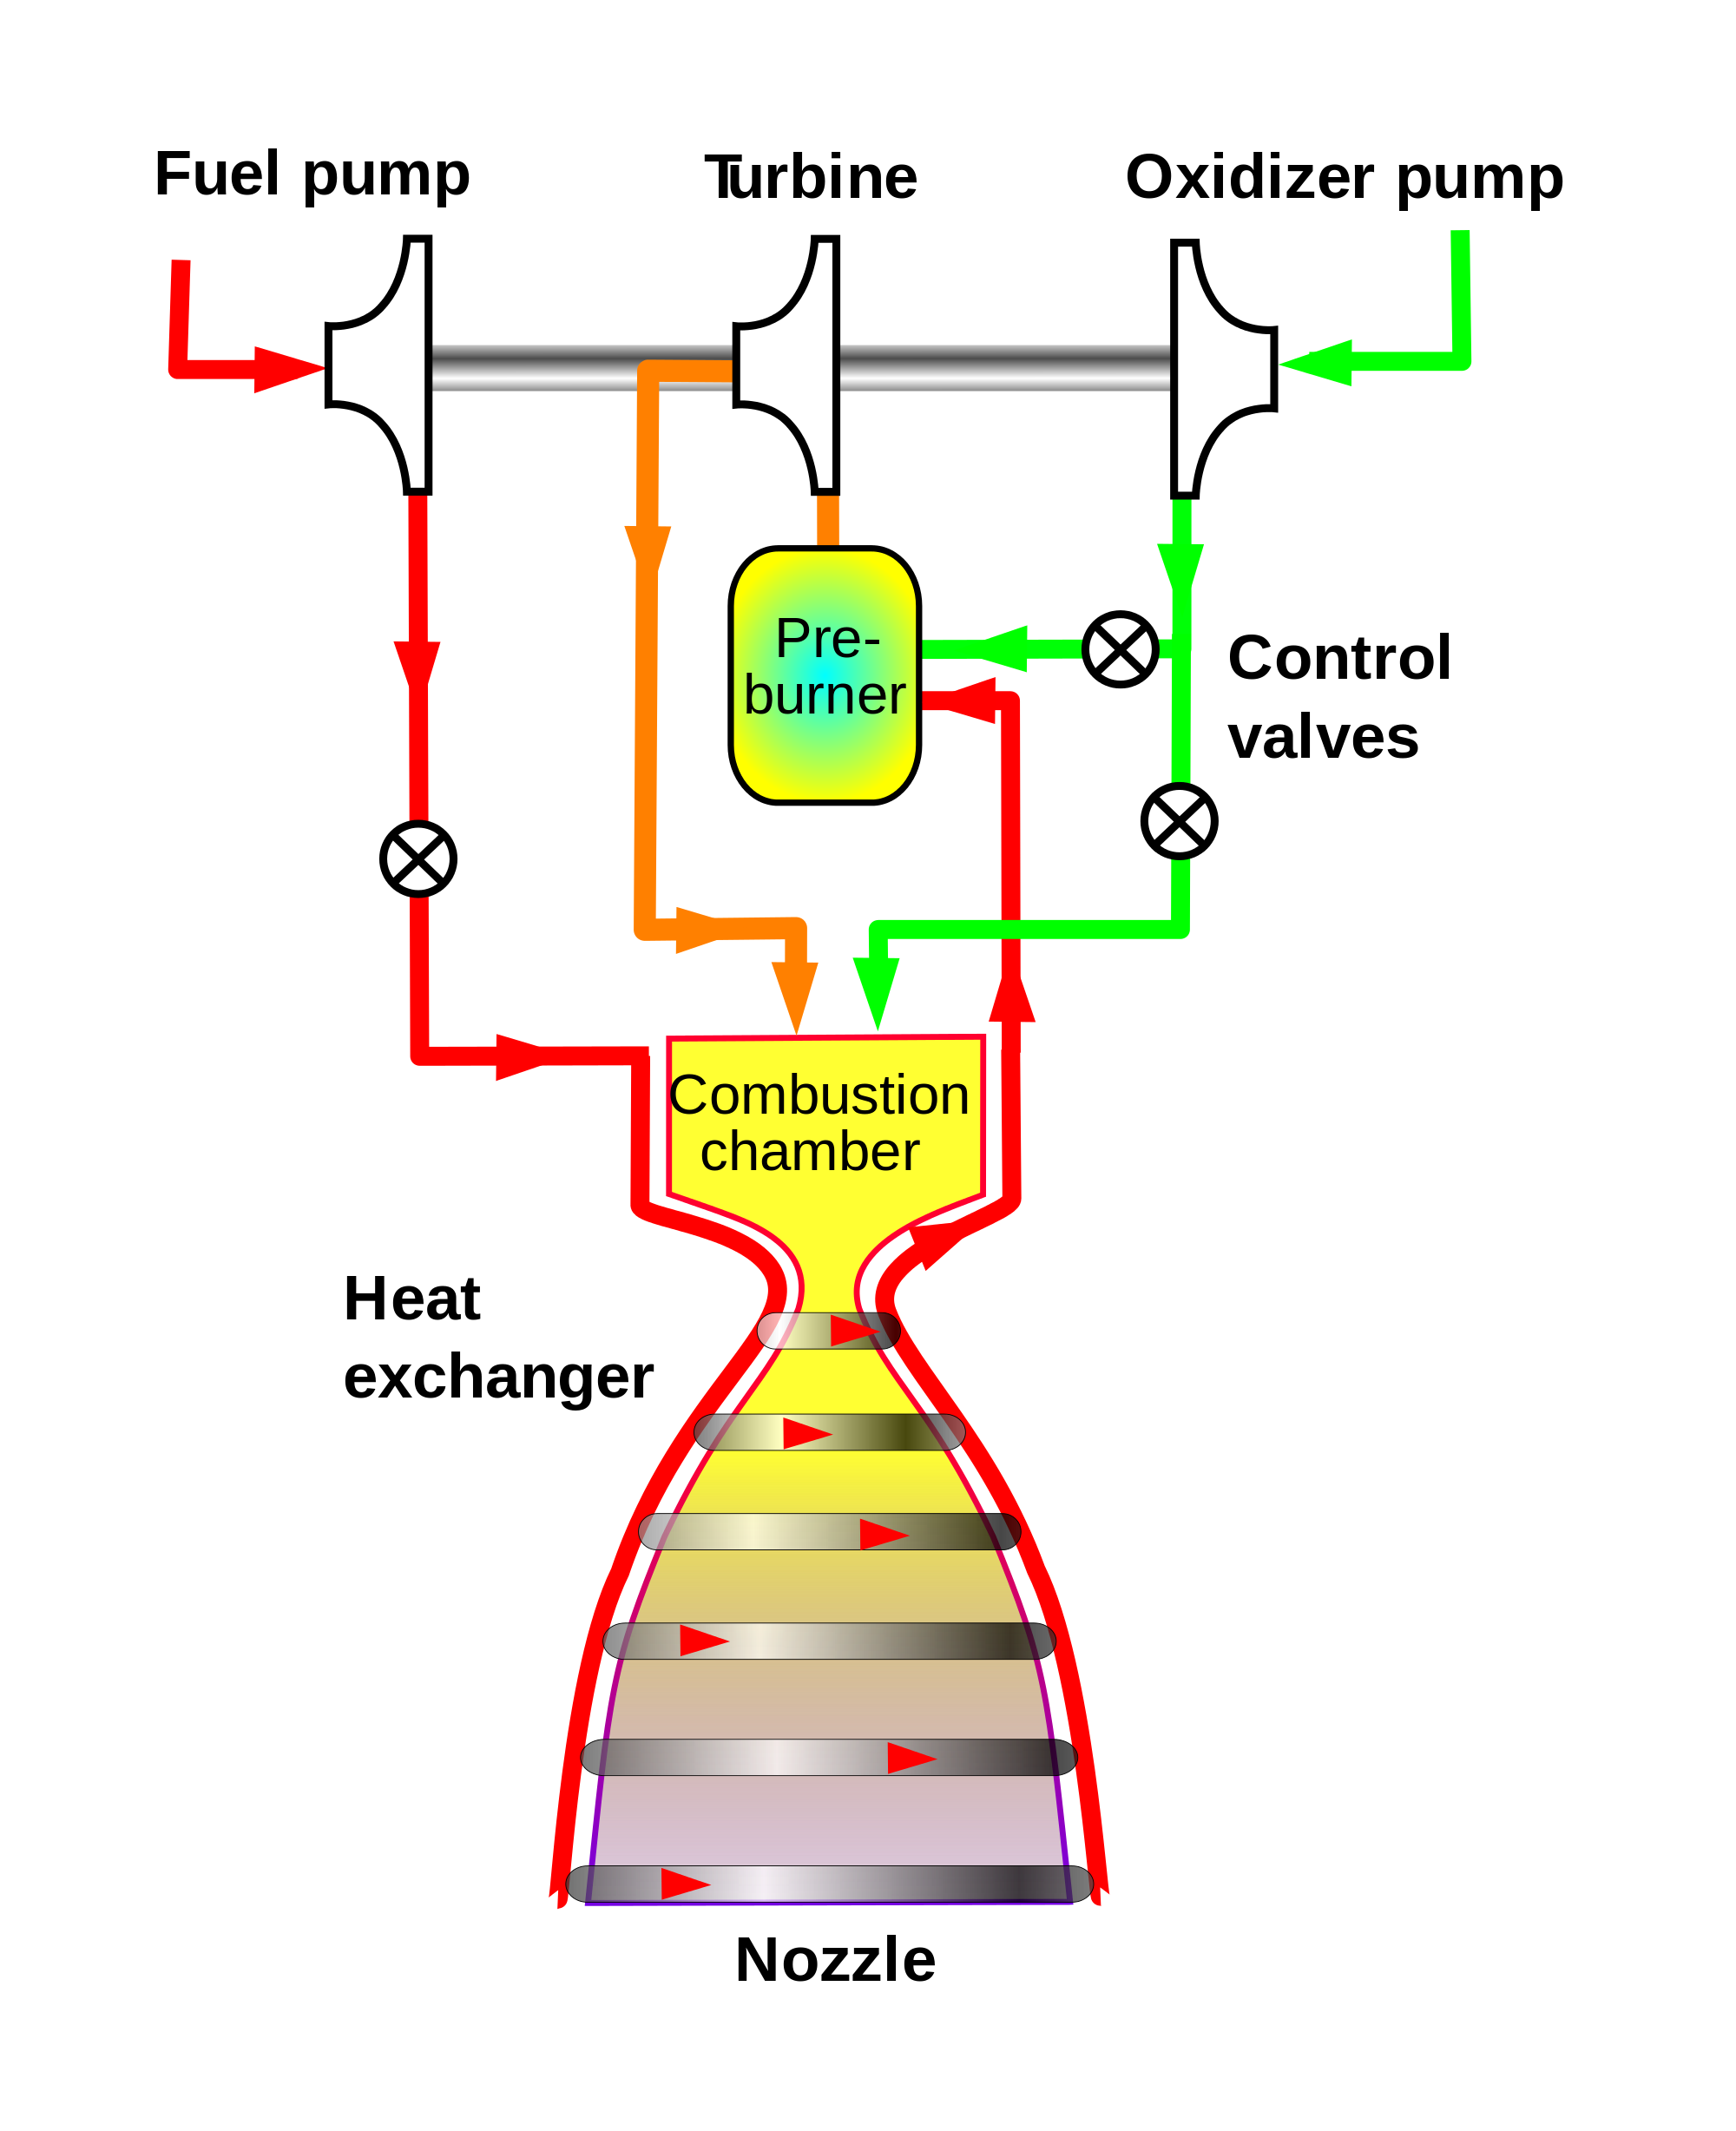
\includegraphics[width=0.35\textheight, angle=0,origin=c]{chapter_1/Staged_combustion_rocket_cycle.svg.png}
    \caption{Принципова схема РРД закритого циклу (англ. closed cycle engine)}
    \label{fig:closed_cycle}
\end{figure}

Тиск на виході турбіни в такому двигуні вищий, ніж у камері згоряння РРД, а на вході в газогенератор, що приводить в рух турбіну, --- ще вище. Щоб задовольнити ці вимоги, для приводу турбіни використовуються ті ж компоненти палива (під високим тиском), на яких працює сам РРД (з іншим співвідношенням компонентів, як правило, -- з надлишком пального, щоб знизити теплове навантаження на турбіну).

Альтернативою замкнутому циклу є відкритий цикл, при якому вихлоп турбіни викидається прямо в навколишнє середовище через відвідний патрубок (рис.~\ref{fig:gas_generator}).

\begin{figure}
    \centering
    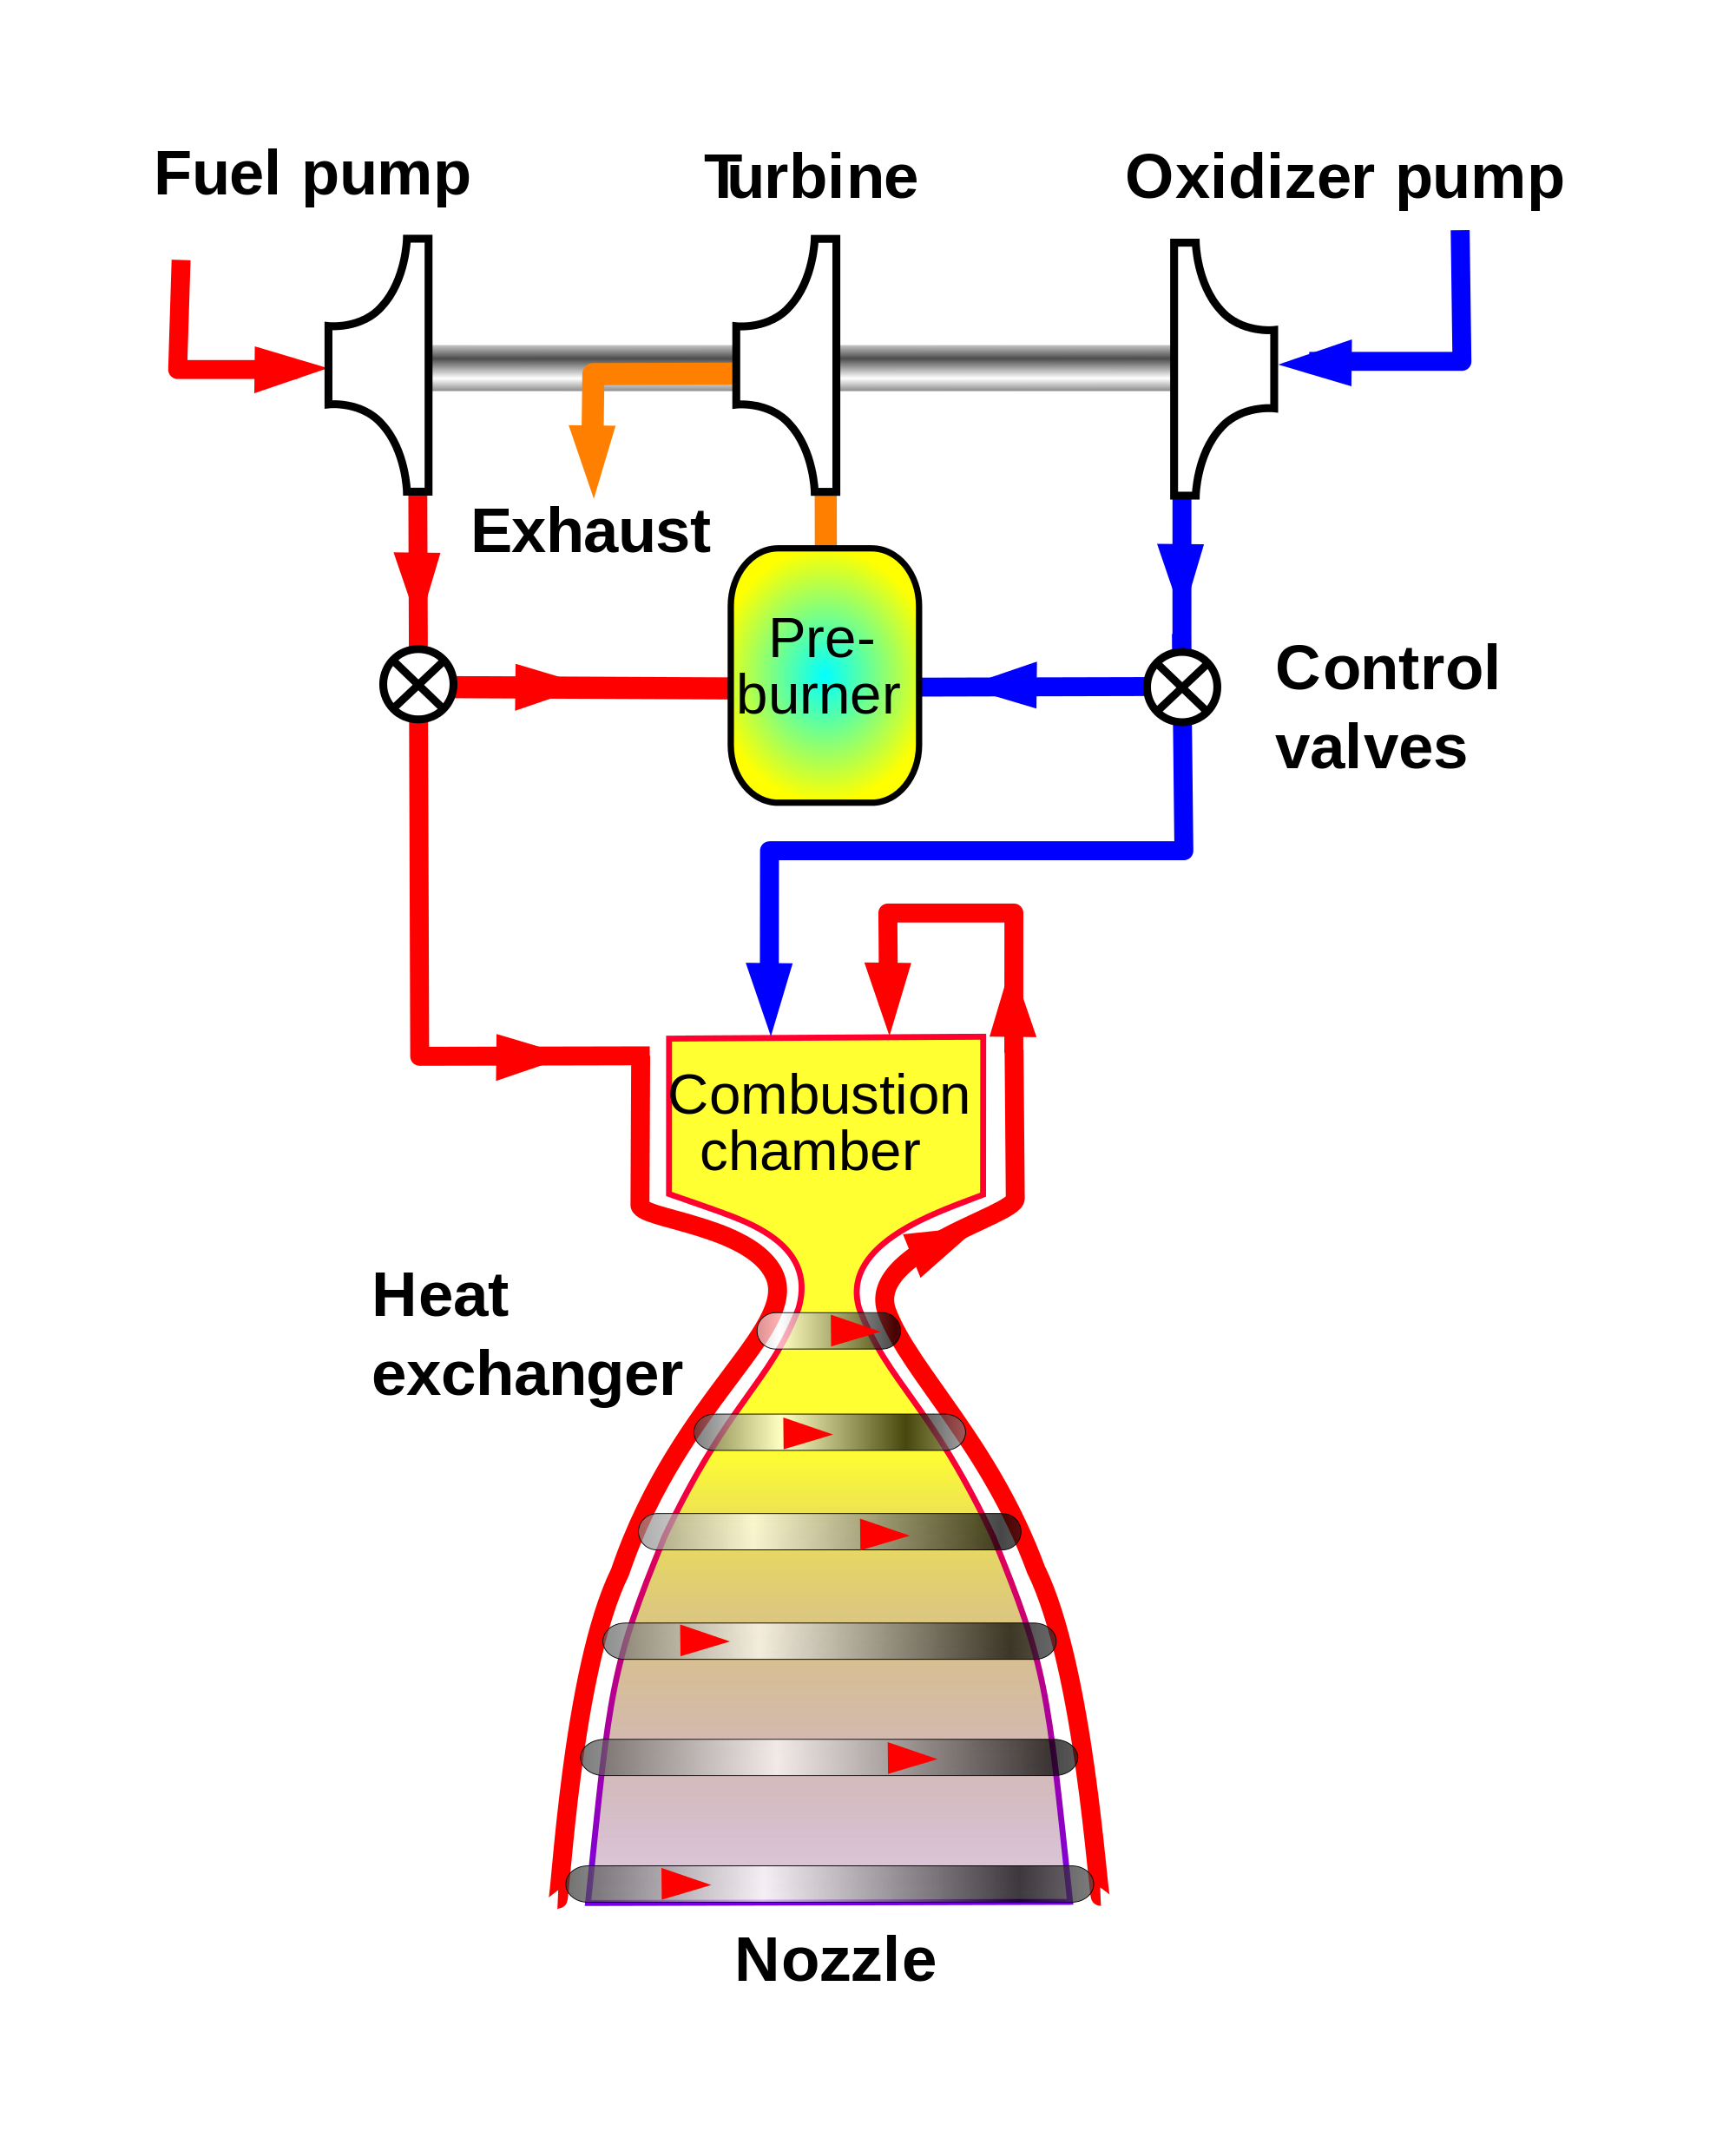
\includegraphics[width=0.35\textheight, angle=0,origin=c]{chapter_1/Gas_generator_rocket_cycle.svg.png}
    \caption{Принципова схема РРД відкритого циклу (англ. gas generator cycle engine)}
    \label{fig:gas_generator}
\end{figure}

Реалізація відкритого циклу технічно простіша, оскільки робота турбіни не пов'язана з роботою камери РРД, і в цьому випадку ТНА взагалі може мати свою незалежну паливну систему, що спрощує процедуру запуску всієї рушійної установки. Але системи з замкнутим циклом мають трохи кращі значення питомого імпульсу, і це змушує конструкторів долати технічні труднощі їхньої реалізації, особливо для великих двигунів ракет-носіїв, до яких пред'являються особливо високі вимоги за цим показником.

При невеликій тязі двигуна (і, отже, невеликій витраті палива) турбонасосний агрегат стає занадто важким елементом, що погіршує масові характеристики рушійної установки. Альтернативою насосній паливній системі служить витискувальна, при якій надходження палива в камеру згоряння забезпечує тиск наддуву в паливних баках, створюваний стисненим газом, найчастіше азотом, який є незаймистим, неотруйним, не є окиснювачем і порівняно дешевий у виробництві (рис.~\ref{fig:pressure_fed}).

\begin{figure}
    \centering
    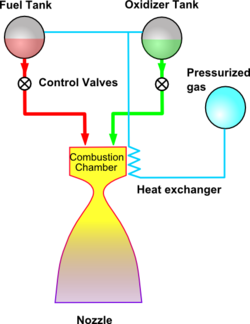
\includegraphics[width=0.4\textheight, angle=0,origin=c]{chapter_1/Pressure_fed_rocket_cycle.png}
    \caption{Принципова схема РРД з витискувальною подачею палива (англ. pressure-fed engine)}
    \label{fig:pressure_fed}
\end{figure}

Для наддуву баків з рідким воднем використовується гелій, оскільки інші гази при температурі рідкого водню конденсуються і перетворюються в рідини~\cite{Dorofeyev}.

Аналогом газогенераторного циклу є інша схема роботи РРД, двигун такої схеми і розглядатиметься  у ході роботи --- цикл з фазовим переходом (англ. expander cycle) (рис.~\ref{fig:expander_cycle}).

\begin{figure}
    \centering
    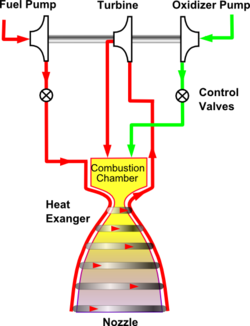
\includegraphics[width=0.4\textheight, angle=0,origin=c]{chapter_1/Expander_rocket_cycle.png}
    \caption{Принципова схема циклу РРД з фазовим переходом (безгазогенераторний РРД) (англ. expander cycle engine)}
    \label{fig:expander_cycle}
\end{figure}

Принцип роботи циклу з фазовим переходом полягає у збільшенні енергії потоку пального (а також окиснювача у деяких варіантах виконання) за рахунок тепла, виділеного камерою згоряння. Тепло передається охолоджуючим кожухом, розташованим навколо КЗ і сопла. Потік, що увібрав теплоту, направляється у ТНА, який відбирає частину енергії потоку для розкрутки турбін пального і окиснювача. Щойно випущений з ТНА потік впорскується в КЗ і згоряє у випадку закритого циклу з фазовим переходом, або ж викидається з контура у варіанті відкритого циклу. Зазвичай у таких установках використовуються кріогенні паливні компоненти, наприклад рідкі водень (\ce{LH2}) та кисень (\ce{LOX}).

Функція турбонасоса у такому циклі полягає у збільшенні тиску у потоці до значення, що компенсує перепад тиску в системі охолодження та контурі загалом, спад тиску внаслідок розширення у турбіні та забезпечує необхідний тиск у форсуночній камері. 

Надійність установок, що використовують цикл з фазовим переходом, забезпечується простотою схеми і відносно малими механічними й тепловими навантаженнями на переріз турбіни. Межа використання такого циклу двигуна пов'язана із значенням температури на вході в турбіну, оскільки площа, яку покриває охолоджувальний кожух, обмежена. Проблема пояснюється законом квадрата-куба: зі зростанням розмірів сопла внаслідок збільшення тяги, площа його поверхні збільшується пропорційно квадрату діаметра, проте об'єм пального, що потрібно нагріти, зростає пропорційно діаметру в кубі. Звідси маємо, що існують максимальні габарити двигуна, поза якими площі поверхні сопла вже не вистачає для нагрівання пального, достатнього для розкрутки ним турбіни і відповідно усього ТНА~\cite[с. 5 -- 6]{Cantiani}.


\section{Процеси, протікаючі в камері згоряння РРД}

Рідинний ракетний двигун є складним пристроєм, у камері згоряння якого протікає не лише екзотермічна реакція окиснення пального, а й низка важливих супутніх явищ, що є взаємопов'язаними: зокрема це газодинамічне прискорення робочого тіла через перепад тисків на вході й виході та його ізобарне нагрівання.

\subsection{Хімічна кінетика: горіння в КЗ}

У типовому рідинному ракетному двигуні тиск всередині камери згоряння може досягати 200 атмосфер, що є набагато більшим, ніж тиск в інших більш поширених двигунах внутрішнього згоряння, таких як автомобільний чи газотурбінний. Для того, щоб зрозуміти та спрогнозувати процес горіння у РРД, потрібен новий деталізований кінетичний механізм системи \ce{H2 / O2}, оскільки усі моделі, запропоновані до цього часу, не були перевіреними за умов високого тиску, що обмежує їх застосування. Збір експериментальних даних для отримання констант швидкості реакції за таких складних умов сам по собі є задачею, вартою окремого фізико --- хімічного дослідження. Деякі константи можуть бути розраховані теоретично, без використання результатів експерименту. Окрім того, у горінні палива в РРД не задіяний розчинник, водночас в багатьох експериментальних установках для визначення швидкості горіння полум'я чи затримки займання присутні азот чи аргон. Це також ускладнює задачу створення детальної кінетичної моделі, що може описувати процеси в РРД.~\cite[с. 383 -- 384]{Shimizu}

У табл.~\ref{chem_kin_h2} наведена детальна кінетична модель, що в рамках даного дослідження~\cite{Shimizu} включає в себе більшість відомих елементарних реакцій між сполуками та радикалами \ce{H2}, \ce{O2}, \ce{H2O}, \ce{H}, \ce{O}, \ce{OH}, \ce{HO2}, і \ce{H2O2}. Дана модель створювалась із використанням уточнених або перерахованих констант реакцій розроблених у попередній моделі авторства Кітано та ін.~\cite[с. 2355 -- 2362]{Kitano}. У процесі розробки цієї моделі не передбачалось узгодження констант реакцій з перевірочними даними, окрім випадку з \ce{H + OH + M = H_2O + M}. Натомість, ці значення брались з надійних літературних джерел. У першу чергу потрібно було визначити величину показників трикомпонентних взаємодій (англ. third-body efficiencies --- авт.) для \ce{H2}, \ce{O2} і \ce{H2O}, оскільки вони є важливими у рамках моделі та впливають на її точність в умовах високого тиску та відсутності розчинника.~\cite[с. 384 -- 385]{Shimizu}.

Для отримання валідних і верифіковних результатів термодинамічних розрахунків камери гібридної електрохімічної ракетної установки необхідно враховувати кінетику хімічних реакцій компонентів паливної суміші за умов високих температур і тисків РРД у присутності частинок присадки, що може призвести до інтенсифікації або сповільнення цих реакцій у камері згоряння (КЗ) двигуна. Високотемпературні реакції за високих тисків, характерних для РРД, ретельно досліджувались та описані у роботах багатьох авторів, зокрема~\cite{Shimizu} для воднево-кисневої суміші. На практиці для опису таких процесів у галузі застосовуються спеціальні програмні пакети, що враховують особливості термодинаміки КЗ ракетних двигунів. Одним із таких є \texttt{Астра.4/рс}, що дозволяє моделювати дво- і трикомпонентні реакції горіння за визначеними моделями таких процесів при заданому тиску (процеси у камері за визначенням циклу Брайтона ізобарні) та співвідношенні компонентів~\cite{Astra}. Пакет написаний мовою \texttt{Fortran}, для роботи застосовується оболонка у середовищі \texttt{Python}. 


\subsection{Термодинамічний опис}

Камера згоряння (КЗ) --- це частина РД, де відбувається власне процес горіння паливної суміші. Температура горіння палива чи не завжди є більшою, ніж температура плавлення матеріалів стінок камери. Отже, основними проблемами цієї частини двигуна є охолодження та/або обмеження часу роботи окремих вузлів під тепловим навантаженням.

Найчастіше камери згоряння виконуються циліндричної форми, з подальшим звуженням до критичного перерізу сопла уздовж осі симетрії. Форма й об'єм КЗ обираються відповідно до основних керуючих параметрів: необхідного значення об'єму для повного змішування і згоряння паливної суміші, спаду тиску газу уздовж осі для прискорення РТ (має бути мінімальним для мінімізації спаду швидкості витікання, а отже й тяги та питомого імпульсу), величини критичного перерізу, що визначає тиск у камері та відповідно її допустимі габарити за даних характеристик і матеріалів тощо.

Теплота передається до усіх внутрішніх поверхонь та обладнання, що відкриті до потоку розжарених газів, зокрема на плиту інжектора, стінки камери і сопла. Густина теплового потоку у камері залежить від параметрів конкретного двигуна; в основному лише  $0.5\ldots 5$~\% усієї енергії, вивільненої газом, передається у вигляді теплоти на стінки камери. Для типового двигуна тягою 44820 Н (10000 lbf) тепловий потік на стінку КЗ може сягати $0.75 -  3.5$~МВт, в залежності від фактичних умов роботи  й конструкції.

Кількість теплоти, що передається через теплопровідність газу камері є нехтуваною. Найбільшим за часткою є конвективний теплообмін. Частину (зазвичай від 5 до 35\%) становить радіаційна передача теплоти.

За фіксованого параметру тиску у КЗ та збільшенні тяги двигуна площа поверхні зростає менш швидко, ніж об'єм. Тому охолодження камери легше реалізується у великих габаритах установки, водночас у менших двигунах знятий системою охолодження тепловий потік є критично важливим параметром внаслідок дії закону квадрата-куба.

Вищий тиск у камері згоряння спричиняє збільшення питомого імпульсу, поряд з тим збільшуючи масу двигуна. Однак, результуюче збільшення інтенсивності теплообміну зі стінкою часто накладає межі зростання практичного значення тиску у КЗ як для твердопаливних, так і для рідинних РД.

Величина теплового потоку у хімічних РД може варіюватись від менш, ніж $50~W/cm^{2}$ до понад $16~kW/cm^{2}$. Найбільшими є значення у критичному перерізі великогабаритних КЗ та твердопаливних РД високого тиску. Меншими є показники для газогенераторів, ділянок біля зрізу сопла, або малих КЗ малого тиску~\cite[с. 282 -- 286]{Sutton}.

\subsection{Газодинамічні процеси}

У типовому надзвуковому соплі велика частина теплової енергії газу в КЗ перетворюється у кінетичну енергію його руху. Тиск газу і його температура швидко спадають, водночас швидкість може досягати кількох миль за секунду. Це зазвичай є ізоентропійним процесом. Якщо внутрішня стінка сопла має дефект (зварний шов чи скол), кінетична енергія газу локально перетворюється у теплову, причому температура й тиск приймають значення таких для потоку газу у камері, спричиняючи руйнування стінки; отже, вона має бути гладкою і позбавленою нерівностей.

Температура у КЗ в ізоентропійному процесі мало відрізняється від стагнаційної температури (температури горіння у хімічних РД). Швидкість витікання газу з сопла є функцією відношення тисків у КЗ і ззовні, адіабатичного показника продуктів згоряння, а також температури на вході у сопло і газової сталої для даної суміші. Оскільки газова стала пропорційна молярній масі, швидкість витікання (або ж питомий імпульс, має розмірність швидкості) є функцією відношення температури на вході у сопло і молярної маси потоку. Це відношення є важливим для оптимізації масової пропорції компонентів палива.

Максимальна теоретична швидкість витікання є скінченною, попри те, що відношення тисків може бути нескінченно великим; це пов'язано з тим, що внутрішня енергія хімічних сполук приймає скінченне значення; нескінченного розширення відбутись не може, оскільки воно призводить до фазових переходів газу.

У соплах ракетних двигунів можуть бути отримані великі швидкості витікання (більші, ніж  $1$~км/с). Спад температури продуктів згоряння є дуже помітним; уздовж короткого відрізку вона може падати на  $2-3$ порядки. Зі збільшенням кінетичної енергії руху потоку газу зменшується його ентальпія, що пропорційно знижує температуру. Оскільки газ одразу після проходження зрізу сопла усе ще є розжареним (типові температури порядку $1000$ К), він містить істотну кількість тепла, не перетвореного у кінетичну енергію потоку.

Неідеальна поведінка камер і сопел РД тісно пов'язана з присутністю у реальних установках стрибків ущільнення, або ж ударних хвиль, що здебільшого виникають у дифузорній ділянці сопла й існують лише у надзвукових потоках. Хвилі розрідження, що також є суто надзвуковим феноменом, утворюються за зрізом сопла й знижують тиск потоку до значень, відповідних навколишньому середовищу.~\cite[с. 52 -- 69]{Sutton}

\section{МПД-прискорювач: узагальнений опис пристрою}

\begin{figure}
	\centering
	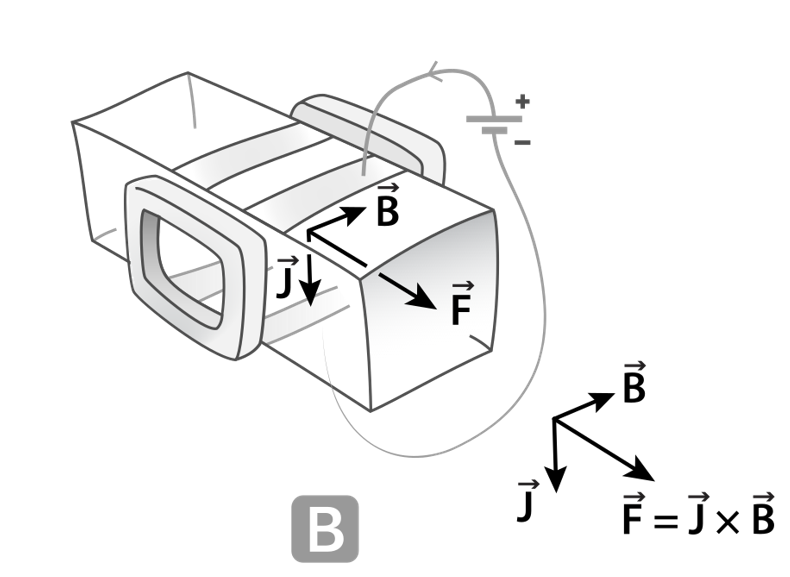
\includegraphics[width=0.6\textheight, angle=0,origin=c]{chapter_1/MHD_thruster_principle.png}
	\caption{Ілюстрація принципу роботи МПД-прискорювача}
	\label{fig:MHD_thruster_principle}
\end{figure}

\begin{figure}
	\centering
	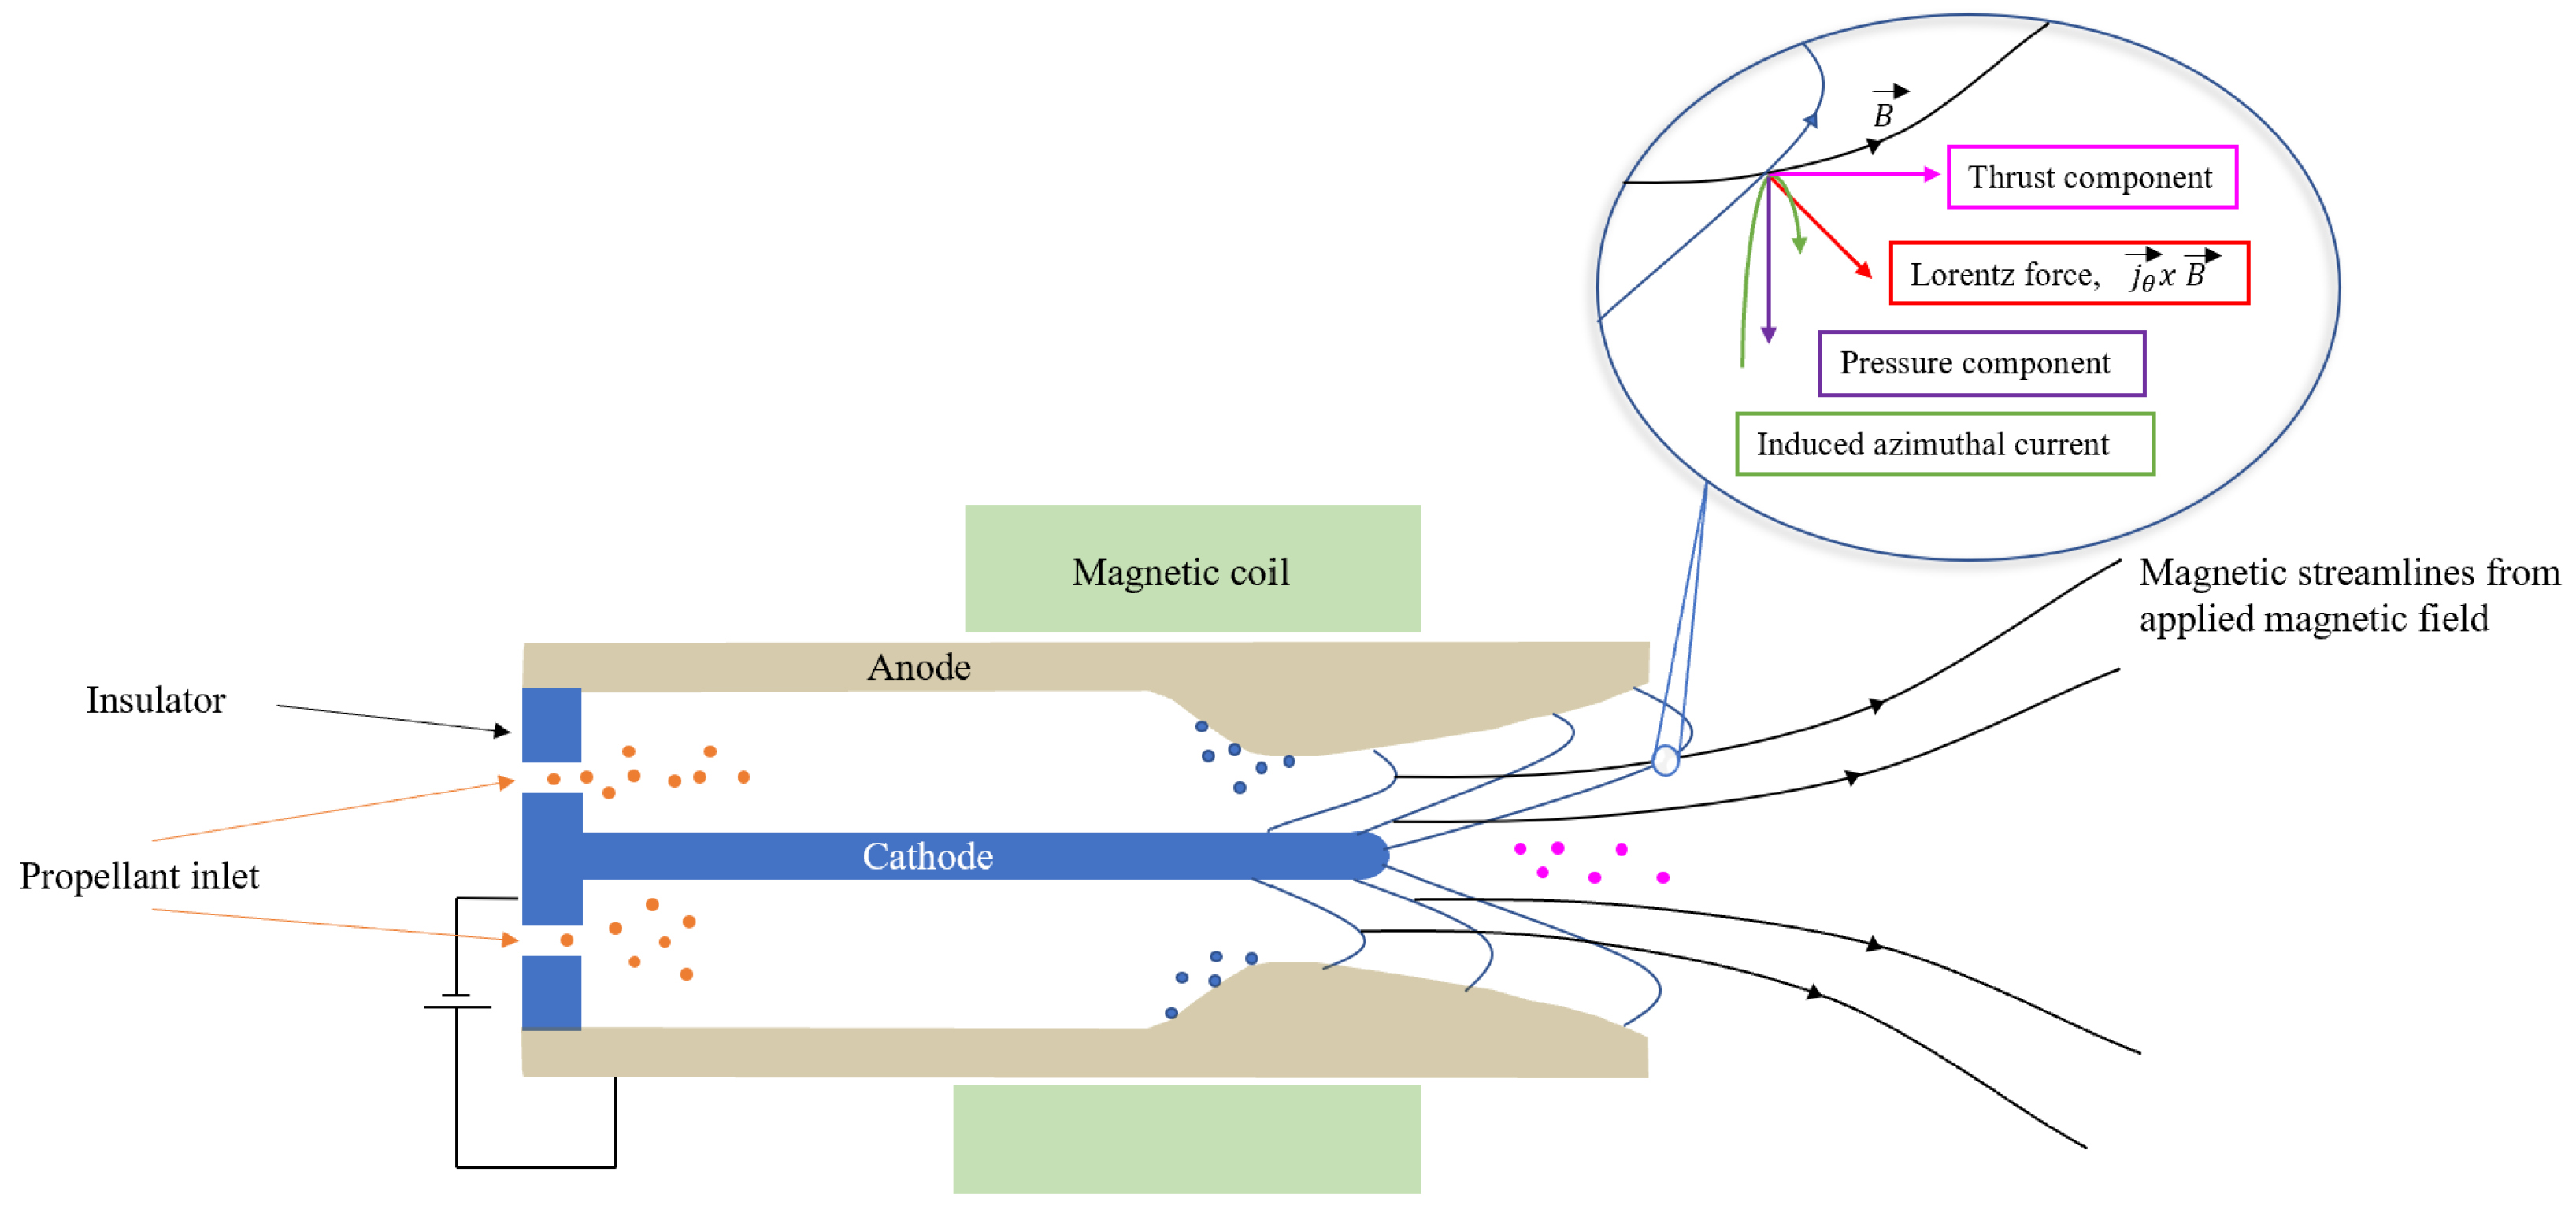
\includegraphics[width=0.6\textheight, angle=0,origin=c]{chapter_1/MHD_thruster_coaxial.jpg}
	\caption{Схема роботи МГД-прискорювача (аналог; катод показаний коаксіальним)}
	\label{fig:MHD_thruster_coaxial}
\end{figure}

Для надання кінетичної енергії потоку робочого тіла (порошок присадки металічного калію, що іонізується у потоці розжареного газу РРД) МПД-прискорювач використовує схрещені електричне та магнітне поля, що створюються протилежно розташованими електродами і котушками з віссю, перпендикулярною до осі каналу, по якому рухається робоче тіло (МПД-канал, він же у плазморідинному двигуні є камерою і соплом РРД) (рис.~\ref{fig:MHD_thruster_principle}). Принципова схема рушійної МГД-установки наведена на рис.~\ref{fig:MHD_thruster_coaxial}; на схемі один з електродів розташований коаксіально, у схемі ж плазморідинного двигуна, що розглядається, обидва електроди розміщені на протилежних стінках МПД-каналу.

В МГД-прискорювачах щільних плазмових середовищ проходить зворотнє до МГД-генератора перетворення виду енергії, тобто електрична енергія, яку ми підводимо, перетворюється в кінетичну і теплову. В каналі МГД-прискорювача відбувається прискорення плазмового середовища під дією пондеромоторної сили (сили Ампера), що дозволяє отримати в лабораторних умовах гіперзвукові швидкості потоку, характерні для аерокосмічних польотів. При швидкостях повітряного чи газового потоку з числом Маха $M > 10$ температура, ентальпія і гальмівний тиск досягають величин, неможливих при спаленні хімічного палива ($> 10$~кК, $>20$~МДж/кг, $\ge 1000$ ат відповідно). МГД-прискорювачі вже знайшли практичне використання у складі аеродинамічних труб для моделювання аерокосмічних польотів та високошвидкісного обтікання тіл (конструкцій).~\cite[с. 10]{Panchenko}

\section{Бар'єр питомого імпульсу існуючих РД}

Основні параметри ракетних двигунів (тяга та питомий імпульс) мають обмеження, пов'язані здебільшого з умовами протікання процесів надання енергії робочому тілу.

Усі розглянуті схеми РРД у більшій чи меншій мірі розв'язують одну й ту ж проблему --- збільшення питомого імпульсу за умови збереження тягооснащеності (додавання газогенератора, замикання контуру пального та окиснювача на камері згоряння тощо); це зводиться до простого підвищення тиску в КЗ, а він у свою чергу залежить від теплоти згоряння пального та тиску в системі перед КЗ, що пов'язані з потужністю ТНА пального та окиснювача; відповідно маємо, що ефективність РРД обмежена максимальною теплотою згоряння в КЗ, або ж у випадку використання газогенератора --- температурою плавлення лопаток його турбіни. Ці параметри зумовлюють обмеження питомого імпульсу двокомпонентних РРД величиною близько $4800$ м/с (близько $490$~с); в істотно важчих з точки зору технічної реалізації трикомпонентних схем рекордне значення досягає $542$ с (паливна суміш літій -- водень -- фтор). 

Виникає потреба усунути або ж компенсувати обмеження швидкості РТ, надавши йому додаткову енергію. Відомо, що за тисків та температур у КЗ набуває істотності процес дисоціації продуктів згоряння та їх часткової іонізації. Ступінь іонізації газу є незначним (близько 1-2 процентів), проте надалі надавати теплоту робочому тілу невигідно, оскільки основний механізм її надання (горіння) переривається внаслідок вищезгаданої рекомбінації реагентів. Поряд із цим надлишкова енергія РТ, що частково йде на іонізацію, у РРД ніяк не використовується. Газодинамічна складова проблеми полягає у неможливості адаптації сопла до широкого діапазону навколишніх тисків; за надто високих значень тиску середовища має місце перерозширення сопла, за малих --- недорозширення; використання соплових насадків є невигідним через відсутність можливості плавної адаптації РД до зміни тиску.

МПД-установки були апробовані в якості двигунів малої тяги для супутників, проте для їх роботи потрібне потужне джерело електроенергії, що зменшує тягооснащеність силової установки до значень, неприйнятних для використання в ролі маршової рушійної установки в межах атмосфери; ця ж проблема постає для всіх існуючих електричних ракетних двигунів.

%Сучасні розроблені ядерні ракетні двигуни, що мають теоретично достатнє для атмосферного використання значення тягооснащеності, діють за принципом реакторних установок з протікаючим крізь активну зону робочим тілом; відповідно РТ такого двигуна є радіоактивним, це зумовлює неможливість його використання в межах атмосфери Землі. Інші схеми роботи ЯРД (рідинно- та газофазні типу "ядерної лампи"), що не передбачають прямого контакту РТ з активною зоною реактора, не можуть бути реалізовані з використанням існуючих матеріалів та технологій.

\section{Плазморідинний ракетний двигун: проблематика і принцип роботи}

Новий тип ракетного двигуна, принцип роботи якого теоретично та чисельно описується у цій роботі, є потенційно ефективнішим, ніж існуючі зразки рідинних ракетних двигунів, і відповідно виступає кращим зразком рушійної установки для верхніх ступеней ракет-носіїв для виведення вантажів по траєкторії з верхніх шарів атмосфери у вакуум на низькі й перехідні орбіти Землі з меншими втратами палива і питомого імпульсу --- це рідинний ракетний двигун з магнітоплазмодинамічним прискорювачем, або плазморідинний ракетний двигун.

Така установка може вирішити проблему ефективного високоатмосферного РД шляхом комбінування РРД та МПД-прискорювача в гібридну установку, що використовує як хімічний/газодинамічний, так і електромагнітний способи надання енергії РТ для збільшення швидкості витікання, а отже і питомого імпульсу.

Рідинні ракетні двигуни мають дуже велику кількість різновидів конструкцій та схем роботи: двигуни з витіснювальною подачею палива, турбонасосні відкритого циклу, закритого циклу з допалюванням окиснювального, генераторного газу тощо~\cite{Dobrovolskiy}. Розглядаючи новий тип гібридного двигуна, варто обирати тип РРД, що відповідає двом показникам: 
\begin{itemize}
	\item якомога більший питомий імпульс;
	\item можливість використання потужності двигуна для живлення МПД-прискорювача.
\end{itemize}


Такими різновидами РРД є безгенераторні двигуни з фазовим переходом (англ. \texttt{expander cycle engine}) та двигуни закритого циклу~\cite{Sutton}. Перші відрізняються відсутністю газогенератора, що полегшує та спрощує конструкцію двигуна, проте позбавляють можливості масштабування через те, що потужність установки обмежується властивостями робочого тіла (палива) --- у безгенераторних двигунів зазвичай використовується водень як пальне з найбільшим відношенням внутрішньої енергії до молярної маси, проте теоретична потужність такого двигуна незначна. Можливість зняття потужності з безгенераторного двигуна відсутня, оскільки уся енергія робочого тіла використовується для розкрутки турбонасосного агрегата (ТНА). 
Двигуни закритого циклу можуть мати значну тягу та питомий імпульс --- їхні характеристики обмежуються допустимим тиском у газогенераторі, що використовується для розкрутки ТНА і має бути більшим за тиск у камері згоряння~\cite{Ovsyannikov}. Проте уся енергія робочого тіла такого РРД використовується для максимізації потужності насосів та збільшення тиску у камері згоряння, що виключає можливість відбору потужності з установки без істотних змін у конструкції газогенератора і турбіни.

Отже, для інтеґрації РРД і МПД-прискорювача без додавання окремої енергоустановки, використовуючи внутрішню енергію палива РРД, необхідно використати цикл і принципову схему двигуна, що передбачатиме наявність окремої газової турбіни, не пов'язаної з ТНА РРД принаймні на його номінальному режимі.

Електромагнітне прискорення РТ вимагає певних значень ступеня його іонізації; продукти згоряння РРД мають високу температуру та достатньо надлишкової енергії через високий тиск у КЗ, проте іонізованих частинок там недостатньо. Для збільшення ступеня іонізації потоку в нього через окрему форсунку на етапі змішування вводиться присадка дрібнодиспергованого калію у розмірі декількох процентів від масової витрати двигуна; калій обраний через його малу енергію іонізації, що зумовлює найбільш повний перехід у потік заряджених частинок, що можуть бути прискорені електромагнітним полем МПД-каналу; у моделях, що розглядаються у розділі~\ref{sec:model_conditions}, вхідний переріз потоку з паливом РРД спільний. МПД-канал згідно такої схеми подачі присадки розташовується у закритичному перерізі сопла РРД, що є принциповою відмінністю поряд із конструкціями, що розглядались у попередніх роботах~\cite{Previous}.


\section{Висновки до розділу \ref{sec:First}}

Проведений аналіз літературних джерел показав, що рідинні ракетні двигуни мають межу ефективності, пов'язаний з бар'єром питомого імпульсу цих установок --- кінетична енергія руху обмежується внутрішньою енергією паливних компонентів, а зовнішнє підведення енергії відсутнє, що призводить до зменшення ефективності використання літальних апаратів з цими двигунами.

Запропонована принципова схема плазморідинного ракетного двигуна потребує належного числового моделювання термодинаміки процесів у ньому, для подальшої валідної оцінки її ефективності, потребується змоделювати термо- та газодинаміку потоку робочого тіла РРД і МПД-прискорювача у спільному середовищі. Також необхідно враховувати конструктивні обмеження конфігурації гібридної рушійної установки внаслідок особливостей умов роботи МПД-компонента.

З урахуванням особливостей процесів, розглянутих під час аналізу літературних джерел, результати числового моделювання ТД-процесів у РРД за присутності робочого тіла МПД-установки дозволять кількісно оцінити ефективність поєднання РРД і МПД-прискорювача у межах однієї рушійної установки. 